\chapter{Introduction}

\section{Statement of problem}

Our task is to analyse the performance of an application that is soon to be released. A common scenario for system performance consultants is to be first engaged at the end of a project when it is realized that the software is far less responsive than expected. The assignment that where are presented with is an attempt to test students in a similar manner thus we based some of our assumptions on this intent. The separate application components have been tested prior to integration. Our job, as black-box testing engineers, is to asses the performance quality of the application, carry out optimisations to improve run-time performance, explain causes of any prolems and performance issues, and formulate a model of the system. We have to produce a report that has two target audiences executives, for whom an non-technical executive summary will be written, and developers, for whom a technical report will be produced.

\section{Application structure}

The JEE application is based on the AdaptiveCells/J tool (a benchmarking system)\footnote{see apendices for details of AdaptiveCells/J}, with ten configurations/use-cases (config1 to config10). There are a total of seven beans in the application (TB1 to TB7) - see figure \ref{fig_bean_calling}.

Each bean in the AdaptiveCells/J test-bed can call two beans (which can then subsequently also call two beans and so on). The calling sequence for each configuration can be determined from figure \ref{fig_bean_calling}.

We used JBoss as our JEE implementation as it is well established, documented, and we had used this during the other practical sessions. See appendices for exact configurations.


\section{Key Performance Scenarios}
In order a line our evaluation efforts with important use cases we define a number of common sets of interactions. 

\subsection{Use Cases}
As the AdaptiveCells/J is built to simulate different system behaviors defined by the calling paths of a number of EJBs, we will conveniently use each config to represent a use case. Each of these calling paths is invoked by a request to a URL and we can therefore simulate them with one HTTP transaction to a single URL.

\begin{center}
\begin{tabular}{| c | c |}
\hline
Use Case ID & URL \\
\hline
Config1 & /adaptivecellsj/testbed\_servlet?configName=config1 \\ 
Config2 & /adaptivecellsj/testbed\_servlet?configName=config2 \\ 
Config3 & /adaptivecellsj/testbed\_servlet?configName=config3 \\ 
Config4 & /adaptivecellsj/testbed\_servlet?configName=config4 \\ 
Config5 & /adaptivecellsj/testbed\_servlet?configName=config5 \\ 
Config6 & /adaptivecellsj/testbed\_servlet?configName=config6 \\ 
Config7 & /adaptivecellsj/testbed\_servlet?configName=config7 \\ 
Config8 & /adaptivecellsj/testbed\_servlet?configName=config8 \\ 
Config9 & /adaptivecellsj/testbed\_servlet?configName=config9 \\ 
Config10 & /adaptivecellsj/testbed\_servlet?configName=config10 \\ 
\hline
\end{tabular}
\end{center}

\subsection{Workload Intensity}

To define the workload for this application we must make some random assumptions as to the nature of the application and the envirnoment in which it exists.

\begin{itemize}
\item We assume that the application is an in-house line of business application and the load on the application correlates to a dgreee with office hours. 
\item We assume that maximum number of conncurrent users is a factor of the number of employees in the organisation and therefore in the short-term growth in the upper bound is limited. 
\item We assume, because the application is in-house and the vast majority of users are on-site, that the connection speed are typical of a 100mbit ethernet. However we shall monitor bandwidth usage with a view to supplying data for any possible future decisions regarding remote access.
\item We assume that this is a new system that the hardware and software use in the test enviroment is a exactly the same as will be used in the production.
\end{itemize}

Using the assumptions above and aributarily setting the number of employees of our fictitious organization at 1600, we define the following likely loads;

\begin{center}
\begin{tabular}{| c | c | c |}
\hline
Load Name & Time Frames & Users \\
\hline
Off-peak  & 7pm - 7am &  150 \\ 
Normal  & 7am - 2pm, 4pm - 7pm &  500 \\ 
Peak & 2pm - 4pm &  1000 \\ 
\hline
\end{tabular}
\end{center}


\section{Performance Objectives}
We must specify quantitive criteria for evaluating the performance characteristics of our key performance scenarios. Based on research into computer human interaction~\cite{Speeds} we define the maximum expectable response time as 8 seconds, this  includes the loading of the content within the browser. We conveniently set the same response constraint for all our use cases and workloads. Responses that are not recevied within this time will be deemed to be failures.

\section{Execution Environment}
In order to get an accurate picture of how the production system will perform in it important that the test environment is as close to the production system as possible. 

Note: In order to create an environment that simulates our hypothetical context using limited resources we opted to use a relatively low spec servers which would be more easily stress tested with one test client.

\begin{figure}[h]
\centering
\scalebox{0.65}{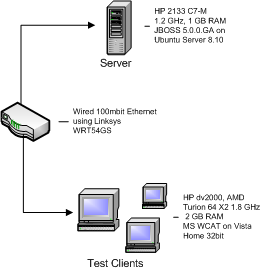
\includegraphics{Graphics/PTE.png}}
\caption{Testing Environment}
\label{fig:4.1}
\end{figure}


\section{Scope}

Our tasks include:
\begin{itemize}
 \item Carry out functional testing and report on any agressive memory leaks and exception occurences;
  \item Load test the application under for a range of typical user loads, measure both client and server side metrics (including garbage collection);
 \item Stress test the application, and identify the threshold where acceptable performance is not attained;
 \item Identify the best stress-resistant configuration;
 \item Carry out optimisation of the JVM, Application Server, and other parameters to improve run-time performance of the application;
 \item Construct three model that closely match the perfromance of observed results.
\end{itemize}

\begin{figure}[h]
% 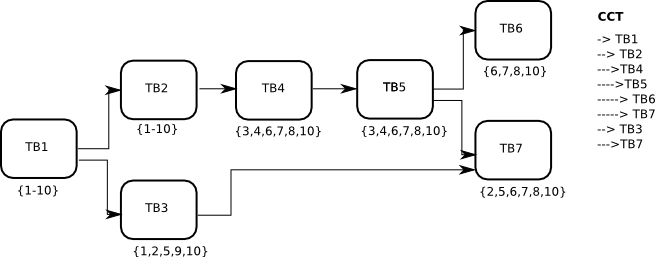
\includegraphics[bb=0 0 524 206]{Graphics/bean_diagram.png}
\scalebox{0.65}{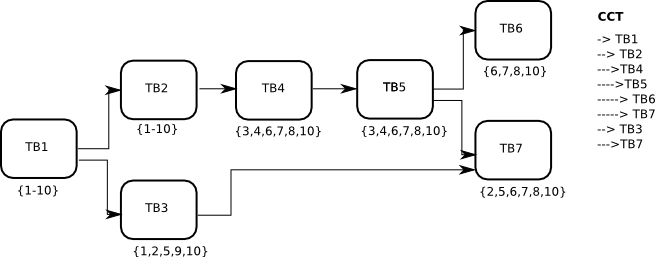
\includegraphics[bb=0 0 524 206]{Graphics/bean_diagram.png}}
 \caption{Bean calling sequence for config1...config10}
 \label{fig_bean_calling}
\end{figure}

